%\documentclass{beamer}

\documentclass[]{beamer}
%\usepackage{pgfpages}
%\pgfpagesuselayout{2 on 1}[a4paper,border shrink=5mm]
%\setbeameroption{show notes}

\usepackage{ctex}
\usepackage{siunitx}
\usepackage{graphicx}

\usepackage[
backend=biber,
style=numeric,
citestyle=ieee,
bibencoding=utf8,
]{biblatex}             %
\addbibresource{main.bib}

\setbeamertemplate{caption}{\raggedright\insertcaption\par}


\usetheme{Montpellier}
\usecolortheme{dolphin}

\title{大跨越输电塔线体系在龙卷风作用下的响应分析}
\author{140926~王勇}
\institute{东南大学}
\date{\today}

\begin{document}

\begin{frame}
	\titlepage
\end{frame}

\section*{目录}
\begin{frame}
  \tableofcontents
\end{frame}

\section{立题依据及价值}
\subsection{输电塔结构特点}
\begin{frame}
  \frametitle{输电塔结构特点}
  \begin{itemize}
  	\item<1-> 输电塔线体系是重要的生命线电力工程设施。
  	\item<2-> 大跨越输电塔线体系具有塔体高、跨距大、柔性强等特点,在极端环境条件(如龙卷风、地震等)下反应敏感,容易发生倒塌破坏。
  	\item<3-> 输电塔线体系的破坏将导致供电系统的瘫痪甚至引发火灾等严重后果。
  \end{itemize}
  
  \begin{block}<4-> {因此,研究大跨越输电塔线体系在各种极端环境条件作用下的静、动态响应,对提高其安全可靠性有着重要的研究及工程应用价值。}
  \end{block}
\end{frame}

\subsection{龙卷风简介}
\begin{frame}
  \frametitle{龙卷风简介}
  \begin{itemize}
  	\item<1->
  	  龙卷风是一种伴随着高速旋转的漏斗状云柱的强风涡旋,中心附近风速可达
  	  \SI{100}{m/s} \textasciitilde{} \SI{200}{m/s},最大可达\SI{300}{m/s}。
  	\item<2->
  	  目前输电塔线体系的抗风研究中,通常仅考虑平均风和脉动风的作用,相关标准或规范尚未包括抗龙卷风的设计要求。
  	\item<3->
  	  国外一些学者已经开始研究龙卷风对输电塔体系的作用。
  \end{itemize}
  \begin{figure}
  	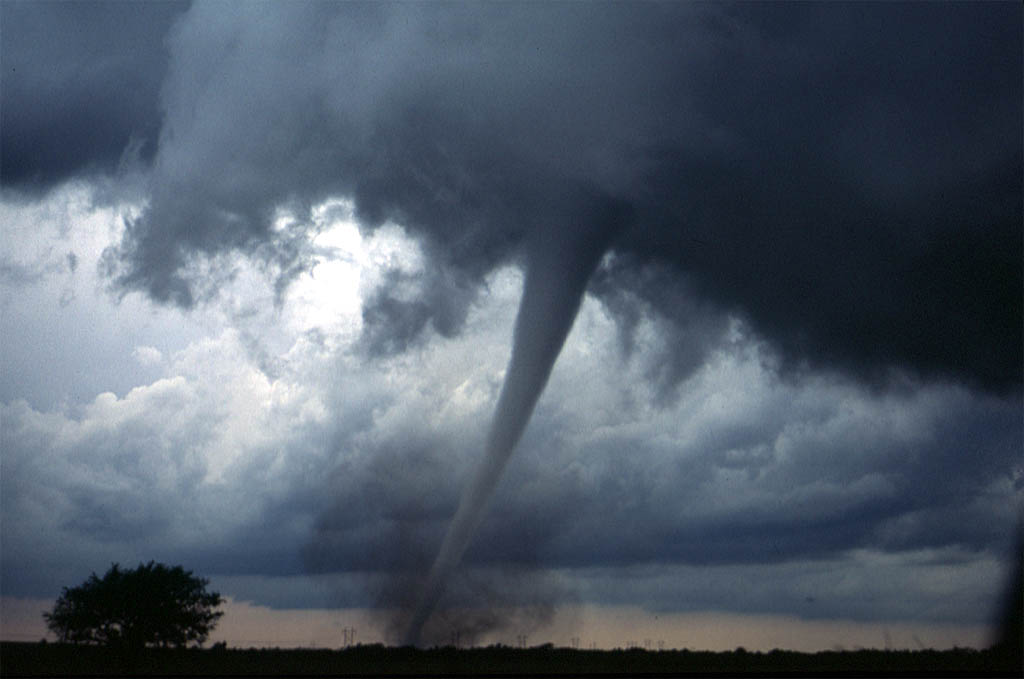
\includegraphics[width=0.6\textwidth]{fig/Dszpics.jpg}
  \end{figure}
\end{frame}

\subsection{输电塔遇龙卷风的倒塌事故}
\begin{frame}
  \begin{figure}
  	\centering
  	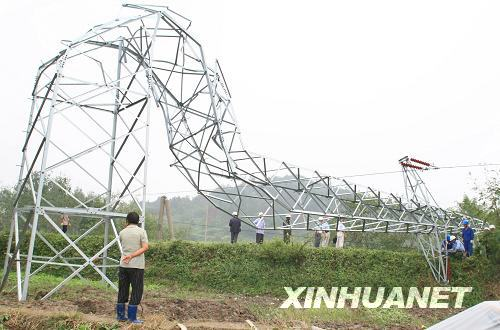
\includegraphics[width=0.8\textwidth]{fig/1.jpg}
  	\caption{2008年9月21日,江苏省宜兴市新街街道等地区遭遇龙卷风袭击,一些高压电线铁塔和电线杆被折断。图为技术人员清理被龙卷风刮倒的高压电线铁塔。来源:新华网\par \url{http://news.xinhuanet.com/photo/2008-09/22/content_10091930.htm}}
  \end{figure}
\end{frame}

\begin{frame}
  \begin{figure}
  	\centering
  	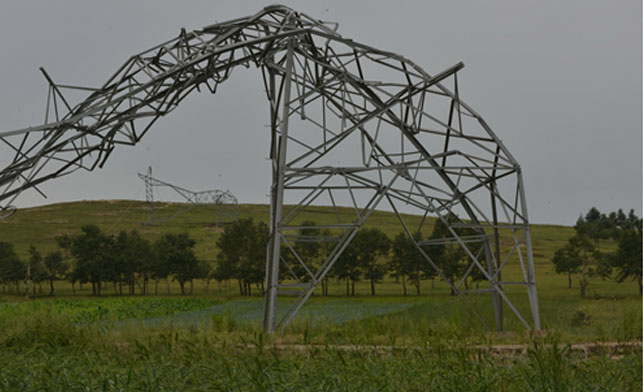
\includegraphics[width=0.8\textwidth]{fig/2.jpg}
  	\caption{2013年7月30日,内蒙古乌兰察布市商都县遭遇龙卷风袭击,多处高压输电塔倒塌。图为龙卷风过后,220千伏输电铁塔拦腰折断。来源:\par \url{http://www.cnjitong.com/jtzt/PicNewsContent.aspx?oid=82}}
  \end{figure}
\end{frame}

\begin{frame}
	\begin{figure}
		\centering
		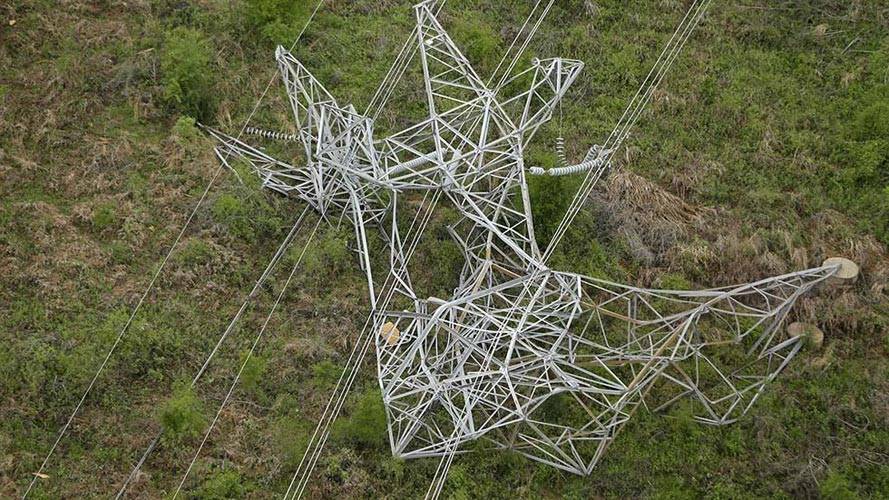
\includegraphics[width=0.8\textwidth]{fig/3.jpg}
		\caption{2014年5月1日,美国阿肯色州五月花市遭受龙卷风袭击,一座输电塔被扭成了“麻花”。来源:中国天气\par \url{http://p.weather.com.cn/2014/04/gqt/2109107.shtml\#p=2}}
	\end{figure}
\end{frame}


\section{研究内容及方法}
\subsection{研究内容}

\begin{frame}
  \frametitle{研究内容}
  \begin{itemize}
  	\item<1->
  	建立龙卷风的计算流体力学模型,并根据实测结果和理论模型验证数值风场的正确性。
  	\item<2->
  	忽略龙卷风的移动,进行输电塔线体系在静止龙卷风风场作用下的静力弹塑性分析,并探讨龙卷风核心位置对输电塔线体系静态响应的影响(参数分析),为设计提供最不利工况。
  	\item<3->
  	考虑龙卷风的移动效应,在典型的龙卷风行进工况下进行输电塔线体系的动力弹塑性分析,并与静力弹塑性分析的结果进行比较,对输电塔线体系的抗龙卷风设计提供参考建议。
  \end{itemize}
\end{frame}

\subsection{研究思路}
\begin{frame}
  \frametitle{研究思路}
  \begin{itemize}
  	\item<1->
  	利用计算流体力学软件ANSYS Fluent模拟F2、F4等级的龙卷风风场,并验证其正确性(与Rankine模型、Wen模型、实测结果等进行比较)。
  	\item<2->
  	利用《架空送电线路杆塔结构设计技术规定》的计算公式将龙卷风风场转化为龙卷风荷载(另一种思路:直接在ANSYS Fluent中建立输电塔模型,并提取输电塔模型所受风压)。
  	\item<3->
  	利用ANSYS软件建立典型的输电塔线体系的有限元模型,考虑材料非线性和几何非线性(输电线的P-delta效应)。
  \end{itemize}  
\end{frame}

\begin{frame}
	\frametitle{研究思路}
	\begin{itemize}
		\item<1->	不考虑龙卷风的移动,选定龙卷风核心相对于输电塔的位置,进而确定龙卷风风场及龙卷风风荷载,在输电塔线体系有限元模型中施加龙卷风荷载,进行静力弹塑性分析。改变龙卷风核心位置,进行参数分析,探讨其对输电塔线体系静态响应的影响。
		\item<2->
		考虑龙卷风移动,将龙卷风风场转化为荷载时程,选取典型工况(如龙卷风行进轨迹平行于、垂直于输电线方向等)进行动力弹塑性分析,并与静力弹塑性分析的结果进行比较。
	\end{itemize}  
\end{frame}

\section{可行性分析}
\subsection{文献综述}
\begin{frame}
  \frametitle{文献综述}
  \begin{itemize}
  	\item<1->
  	Savory (2001) 采用龙卷风Wen模型(忽略风场竖向速度),利用风力系数将风场转化为输电塔线体系所受的龙卷风荷载,并考虑了龙卷风的平移,在龙卷风行进路径垂直于输电塔线的典型工况下进行动力弹塑性分析,并根据结构的动态响应分析其破坏形态。
  	\item<2->
  	Langlois (2007) 主要评估了ASCE等提出的多种龙卷风简化荷载模型对输电塔线体系所受响应的影响。其中的龙卷风简化荷载模型假设输电塔身所受的风压是均匀的,并且忽略了风场的竖向分量及风场对输电线的作用。
  	\item<3->
  	任超 (2010) 仅考虑了龙卷风的平移速度和最大切向速度,利用《架空送电线路杆塔结构设计技术规定》的计算公式将其转化为输电塔线体系所受的龙卷风荷载,进行静力弹塑性分析。
  \end{itemize}  
\end{frame}

\begin{frame}
	\frametitle{文献综述}
	\begin{itemize}
		\item<1->
		Hamada (2010) 利用缩尺CFD模型模拟龙卷风风场,利用ASCE No. 74规范提供的计算方法将风场转化为输电塔线体系受到的龙卷风荷载,然后进行静力弹塑性分析。并改变龙卷风核心的位置,分析其对输电塔线体系所受响应的影响。
		\item<2->
	    Altalmasa (2014) 研究思路与Hamada (2010)类似,进行更详尽的参数分析,即龙卷风核心相对于输电塔的角度、距离这两个参数对输电塔受到的最大响应的影响。
	\end{itemize}  
\end{frame}

\subsection{研究现状}
\begin{frame}
  \frametitle{研究现状}
  国外针对龙卷风对输电塔的研究较为充分,但国外的研究成果难以直接用于国内的输电塔线体系的设计和评估,主要原因在于:
  \begin{itemize}
    \item<2->
    国内外的输电塔线体系的形式有所不同,所以需要针对中国常见的输电塔线体系的典型形式进行建模计算;
    \item<3->
    国内外将风场转化为风荷载的计算公式不同,因此需要利用中国规范或标准的风荷载计算公式评估龙卷风的作用。
  \end{itemize}
\end{frame}

\section{预期的成果}
\begin{frame}
  \frametitle{预期的成果}
  \begin{itemize}
  	\item<1->
  	利用CFD模拟龙卷风风场,并总结针对模拟方法(例如:湍流模型的选择、壁面函数的选择、网格的划分等方面)的经验。
  	\item<2->
  	进行输电塔线体系在静止龙卷风风场作用下的静力弹塑性分析,并探讨龙卷风核心位置对输电塔线体系静态响应的影响(参数分析),分析最不利工况以供设计参考。
  	\item<3->
  	考虑龙卷风的移动效应,在典型的龙卷风行进工况下进行输电塔线体系的动力弹塑性分析,并与静力弹塑性分析的结果进行比较,对输电塔线体系的抗龙卷风设计提供参考建议。
  \end{itemize}
\end{frame}

\section{预计的困难和解决方法} 
\begin{frame}
  \frametitle{预计的困难及解决办法}
  \begin{itemize}
  	\item<1->
  	利用CFD模拟符合实际的龙卷风风场是一个难点,需要对计算流体力学的相关模型较为熟悉。这一困难可通过查阅ANSYS Fluent用户手册,并请教学长等方法解决。
  	\item<2->
  	将CFD模拟的龙卷风风场转化为风荷载并施加到输电塔线体系的有限元模型的过程是难点,因为模型较大,单纯手动输入效率低下且容易出错。这一困难可利用ANSYS APDL语言编程实现荷载施加过程的自动化。
  \end{itemize}
\end{frame}


\section*{谢谢}
\begin{frame}
	\begin{figure}
		\centering
		
\includegraphics[width=\textwidth]{./fig/thank_you.jpg}
	\end{figure}
\end{frame}

\end{document}